\documentclass{lms}
\usepackage[utf8]{inputenc}
\usepackage[american]{babel}
\usepackage[T1]{fontenc}
\usepackage{amssymb,amsmath,amsfonts}
\usepackage{algorithmic}
\usepackage{algorithm}
\usepackage{tikz}
\usepackage{nicefrac}
\usepackage{hyperref}
\usepackage{unicode}
\usepackage{stmaryrd}
 
\newcommand{\todo}[1]{{\color{red}TODO: #1}}
\def\snote#1{}


%\theoremstyle{plain}
\newtheorem{thm}{Theorem}[section]
\newtheorem{lem}[thm]{Lemma}
\newtheorem{cor}[thm]{Corollary}
\newtheorem{prop}[thm]{Proposition}

\newnumbered{defi}[thm]{Definition}
\newnumbered{rem}{Remark}
\newnumbered{exe}{Example}
\newnumbered{prob}{Problem}

\def\mat#1{\begin{pmatrix}#1\end{pmatrix}}
\def\smat#1{{\def\arraystretch{.7}\mat{#1}}}
\def\pa#1{\left(#1\right)}
\def\acco#1{\left\{#1\right\}}
\def\bcro#1{\left\llbracket#1\right\rrbracket}
\def\chev#1{\left\langle#1\right\rangle}
% pour les coûts des opérations M, F etc. (?)
\def\cout#1{\mathsf{#1}}
% let's decide on one!
\let\leq\leqslant \let\geq\geqslant
\def\sfdiv{\mathsf{divide}}

\newcommand{\M}{\mathsf{M}}
\newcommand{\Z}{\mathbb{Z}}
\newcommand{\F}{\mathbb{F}}
\newcommand{\Q}{\mathbb{Q}}
\newcommand{\C}{\mathbb{C}}
\newcommand{\tildO}{\tilde{O}}
\newcommand{\MM}{\cout{M}}
\newcommand{\FF}{\cout{F}}
\newcommand{\RR}{\cout{R}}
\DeclareMathOperator{\loglog}{loglog}

\def\algorithmicrequire{\textbf{Input:}}
\def\algorithmicensure{\textbf{Output:}}

\makeatletter
\def\full@line{8pt}
\def\doublefull@line{12pt}
% \def\@nprf{% nprf environment modified OT 12/11/02
%   \list{}{\topsep 8pt \leftmargin 0pt
%   \itemindent\parindent \labelsep .5em 
%   \listparindent\parindent
%   \settowidth\labelwidth{{\normalfont\rmfamily(iii)}}}%
%   \item{\normalfont\itshape\proofname.}\advance\itemindent\labelsep%
%   \advance\itemindent\labelwidth%
%   \hskip 1em\normalfont\rmfamily\ignorespaces}
\makeatother


% Colors after XKCD color name survey
\definecolor{purple}{rgb}{.49,.11,.61}
\definecolor{green}{rgb}{.08,.69,.10}
\definecolor{blue}{rgb}{.01,.26,.87}
\definecolor{pink}{rgb}{1,.5,.75}
\definecolor{brown}{rgb}{.39,.21,.00}
\definecolor{red}{rgb}{.89,0,0}
\definecolor{lightblue}{rgb}{.58,.81,.98} 
\definecolor{teal}{rgb}{0,.57,.52}
\definecolor{orange}{rgb}{.97,.45,.02}
\definecolor{lightgreen}{rgb}{.53,.99,.01}
\definecolor{magenta}{rgb}{.76,0,.47}
\hypersetup{colorlinks,linkcolor={red!70!black},
  citecolor={green!70!black},urlcolor={blue!70!black}}

\title[Explicit isogenies in any characteristic]{Explicit isogenies in quadratic time in any characteristic}
\author{Cyril Hugounenq}

\classno{11Y40 (primary), 11G20, 14H52 (secondary)}

\extraline{This work was partially supported by the
  \href{http://www.digiteo.fr/}{DIGITEO} grant 2013-0531D (ARGC).}

\begin{document}
\maketitle

\begin{abstract}
The problem we will consider here is the computation of an isogeny between two elliptics curves with the knowledge of the domain and the codomain of the isogeny and it's degree $r$. Couveignes's algorithm is an algorithm which solves this problem in $O(r^2)$ operations using the $p$-torsion. We want to extend the method used by Couveignes  We try to adapt his method here to the case of the $2$ torsion and more generally to the $\ell$ torsion, thus we propose an alternative for medium characteristic with this algorithm.
\end{abstract}

% \section*{Proposed notation}

% This section is for internal reference only: erase after the paper has
% stabilized.

% \begin{itemize}
% \item $\mathbb{F}_q$ is the field we are working on
% \item $\ell$ is for the $\ell$ torsion we are working on
% \item $r$ is the degree of the isogeny we want to compute
% \item $k$ is the integer such that $\ell^{2k}>4r+1$
% \item we thus work with a tower which has for top level $F_{q^{\ell^k}}$
% \item $E$ is for ordinary elliptic curves defined over the finite field $\mathbb{F}_q$
% \item $\mathcal{O}$ (resp. $\mathcal{O}_x$) is the notation for the endomorphism ring associated (up to isomorphism) to $E$ (resp. $E_x$)
% \item $K$ is the notation for the imaginary quadratic field in which $\mathcal{O}$ is defined
% \item $d_K$ is the negative integer such that $K=\mathbb{Z}[d_K]$  
% \end{itemize}

%%%%%%%%%%%%%%%

\section{Introduction}
\label{sec:introduction}

Isogenies are non-zero morphisms of elliptic curves, that is,
non-constant rational maps preserving the point at infinity. They are
also algebraic group morphisms. Isogeny computations play a central
role in the algorithmic theory of elliptic curves. They are notably
used to speed up Schoof's point counting
algorithm\cite{schoof85,atkin88,elkies92,schoof95,elkies98}. They are
also widely applied in cryptography, where they are used to speed up
point multiplication~\cite{gallant+lambert+vanstone01,birkner+sica11},
to perform cryptanalysis~\cite{mauer+menezes+teske01}, and to
construct new
cryptosystems~\cite{teske06,charles+lauter+goren09,Stol,defeo+jao+plut12,jao+soukharev2014-signatures}.

The \emph{degree} of an isogeny is its degree as a rational map. If an
isogeny has degree $r$, we call it an $r$-isogeny, and we say that two
elliptic curves are $r$-isogenous if there exists an $r$-isogeny
relating them. Accordingly, we say that two field elements $j$ and
$j'$ are $r$-isogenous if there exist $r$-isogenous elliptic curves
$E$ and $E'$ such that $j(E)=j$ and $j(E')=j'$. The
\emph{explicit isogeny} problem has many incarnations. In this paper,
we are interested in the variant defined below.

\begin{prob}[(Explicit isogeny problem)] \label{prob:isogeny-problem}
  Given two $j$-invariants $j$ and $j'$, and a positive integer
  $r$, determine if they are $r$-isogenous. In that case, compute
  curves $E$, $E'$ with $j(E)=j$ and $j(E')=j'$, and the
  kernel of an $r$-isogeny $ψ:E\to E'$.
\end{prob}

Once the kernel of the isogeny is computed, the rational maps
associated to it can be computed in optimal time using Velu's
formulas~\cite{velu71}.

This paper focuses on the explicit isogeny problem for \emph{ordinary}
elliptic curves over finite fields. A famous theorem by Tate states
that two curves are isogenous over a finite field if and only if they
have the same cardinality over that field. The explicit isogeny
problem stated here appears naturally in the Schoof-Elkies-Atkin point
counting algorithm (SEA). There, $E$ is the curve of which we want to
compute the cardinality, and $E'$ is an $r$-isogenous curve, with $r$
a prime of size approximately $\log\#E$. For this reason, the explicit
isogeny problem is customarily solved without prior knowledge of the
cardinality of $E$. We will abide by this convention here.

A good measure of the computational difficulty of the problem is given
by the isogeny degree $r$. Indeed the output is represented by
$O(r)$ base field elements, hence an asymptotically optimal algorithm
would solve the problem using $O(r)$ field operations. Many algorithms
have been suggested over the years to solve the explicit isogeny
problem. Early algorithms were due to Atkin~\cite{atkin91} and
Charlap, Coley and
Robbins~\cite{charlap1991enumeration}. Elkies'~\cite{elkies92,elkies98,Bostan}
was the first algorithm targeted to finite fields (of large enough
characteristic). Assuming $r$ is prime, its complexity is dominated by
the computation of the modular polynomial $\Phi_r$, which is an object
of (binary) size $O(r^3\log r)$. Later Bröker, Lauter and
Sutherland~\cite{sutherland10:modpol} optimized the modular polynomial
computation in the context of the SEA
algorithm. Finally Lercier and Sirvent\cite{lercier+sirvent08,1602.00244}
generalized Elkies' algorithm to work in any characteristic. Despite
these advances, the overall cost of Elkies' algorithm and its
variants is still at least cubic in $r$.

Another line of work to solve the explicit isogeny problem was
initiated by Couveignes~\cite{couveignes94,couveignes96,couveignes00},
and later improved by De Feo and Schost~\cite{df10,df+schost12}. These
algorithms use an interpolation approach combined with ad-hoc
constructions for towers of finite fields of characteristic $p$. Their
complexity is quasi-quadratic in $r$, but exponential in $\log p$,
hence they are only practical for very small characteristic.

In this paper we present a variant of Couveignes' algorithm with
complexity polynomial in $\log p$ and quasi-quadratic in $r$. Together
with the Lercier-Sirvent algorithm, they are the only polynomial-time
isogeny computation algorithms working in any characteristic, hence
they are especially relevant for counting points in \emph{medium}
characteristic (i.e., counting points over $\F_{p^n}$, when
$n\gg p/\log p$).

Note that, although Couveignes-type algorithms do not make use of the
modular polynomial $\Phi_r$, its computation is still necessary in the
context of the SEA algorithm. Thus our new algorithm does not improve
the state of the art on point counting \todo{but maybe benchmarks are
  going to show that, at least in practice, we sometimes beat
  Lercier-Sirvent?}. It gives, however, an effective algorithm for
solving the explicit isogeny problem, with potential applications in
other contexts, e.g., cryptography.

\subsection{Notations}

Throughout this paper: $r$~is a positive integer, $p$~an odd prime,
$q$~a power of $p$, and $\mathbb F_q$ is the finite field with
$q$~elements. $E$ ~is an ordinary elliptic curve over~$\mathbb F_q$,
its group of $n$-torsion points is denoted by~$E[n]$, its
$q$-Frobenius endomorphism by~$π$.  The endomorphism ring of $E$ is
denoted by~$\mathcal O$, with~$K = \mathcal O ⊗ ℚ$ the corresponding
number field, $\mathcal O_K$ is its maximal order, and $d_K$~the
discriminant of~$\mathcal O_K$.
For a prime~$ℓ$ different from~$p$ and not dividing~$r$,
we denote by~$E[ℓ^n]$ the group of $ℓ^n$-torsion points of~$E$,
$E[ℓ^{∞}] = \varinjlim E[ℓ^n]$ the reunion of all $E[ℓ^n]$,
and $T_ℓ(E) = \varprojlim E[ℓ^n]$ the $ℓ$-adic Tate module~\cite[III.7]{Sil},
which is free of rank~two over~$ℤ_ℓ$.
The factorization of the characteristic polynomial of~$π$
in~$ℤ_ℓ$ is determined by the Kronecker symbol~$(d_K/ℓ)$.
If $(d_K/ℓ) = +1$ then we also define $λ,μ$ as
the eigenvalues of~$π$ in~$ℤ_ℓ$ and write~$h = v_ℓ(λ - μ)$,
where $v_ℓ$ is the $ℓ$-adic valuation.

We measure all computational complexities in terms of operations in
$\mathbb{F}_q$; the binary costs associated to the algorithms
presented next are negligible compared to the algebraic costs, and
will be ignored. We use the Landau notation $O()$ to express
asymptotic complexities, and the notation $\tildO()$ to neglect
polylogarithmic factors.  We let $\MM(n)$ be a function such that
polynomials in $\F_q[X]$ of degree less than $n$ can be multiplied
using $\MM(n)$ operations in $\F_q$, under the assumptions
of~\cite[Chapter~8.3]{vzGG}. Using FFT multiplication, one can take
$\MM(n)∈ O(n\log n\loglog n)$.

\subsection{Towers of finite fields}
\label{sub:towers}

The algorithms presented next operate on elements defined in finite
extensions of $\F_q$. Specifically, we define a \emph{tower} of finite
fields $\F_q=F₀⊂F₁⊂\cdots⊂F_n$ with $\ell$ dividing $\#F_1-1$, $[F₁:F₀]$
dividing $ℓ-1$, and $[F_{i+1}:F_i]=ℓ$ for any $i>0$. For $ℓ=2$,
we build upon the work of Doliskani and Schost~\cite{DoSc12}. For
general $ℓ$ we use towers of Kummer extensions in a way similar
to~\cite[\S~2]{DeDoSc13}.  Both constructions represent elements of
$F_i$ as univariate polynomials with coefficients in $\F_q$, thus
basic arithmetic operations can be performed with classic modular
polynomial arithmetic. While constructing the tower, we also enforce
special relations between the generators of each level, so that moving
elements up and down the tower, and testing membership, can be done at
negligible cost.

We briefly sketch the construction for odd $\ell$. We first look for a
primitive polynomial $P_1∈\F_q[x]$ of degree equal to $[F₁:F₀]$. There
are many probabilistic algorithms to compute $P_1$ in time polynomial
in $\ell$ and $\log q$; since their cost does not depend on the height
$n$ of the tower, we neglect it. Then, the image $x₁$ of $x$ in
$F_1=\F_q[x]/P₁(x)$ is an element of multiplicative order $\#F₁-1$,
and in particular it is a non $ℓ$-adic residue. Hence for any $i>1$ we
define $F_i$ as $\F_q[x]/P_1\bigl(x^{ℓ^{i-1}}\bigr)$, the computation
of the polynomials $P_1\bigl(x^{ℓ^{i-1}}\bigr)$ incurring no algebraic
cost. Using this representation, elements of $F_i$ can be expressed as
elements of a higher level, and reciprocally, by a simple
rearrangement of the coefficients. Another fundamental operation can
be done much more efficiently than in generic finite fields, as the
following generalization of~\cite[\S~2.3]{DoSc12} shows.

\begin{lem}\label{lemma:frob-ell}
  Let $F_0⊂\cdots⊂F_n$ be a Kummer tower as defined above, and let
  $a∈F_i$ for some $0≤i≤n$. For any integer $j$, we can compute the
  $(\#F_j)$-th power of $a$ using $O(ℓ^i\MM(ℓ) + \MM(ℓ^i))$ operations
  in $\F_q$, after a precomputation independent of $a$ that uses
  $O(ℓ\MM(ℓ)\log(q))$ operations in $\F_q$.
\end{lem}
\begin{proof}
  Without loss of generality, we can assume that $j<i$; otherwise, the
  output is simply $a$ itself. Let $τ=\#F_i$ and $σ=\#F_j$. By
  assumption, $a$ is written as
  $a =a_0 + a_1 x + \cdots + a_{τ-1} x^{τ-1}$, for some $x$ that
  satisfies $x^{\ell^{i-1}}=x_1$, where $x₁∈F₁$ is a root of $P₁$.

  The first step, independently of $a$, is to compute $y=x^σ$. Writing
  $σ = u \ell^{i-1} + r$, with $r < \ell^{i-1}$, we see that $y$ is
  given by $x₁^{u \bmod \#F₁}x^r$. We compute $x₁^{u\bmod\#F₁}$ using
  $O(ℓ\MM(ℓ)\log(q))$ operations in $\F_q$, and we keep this element
  as a monomial of $F₁[x]$.

  Finally, once we know $y$, we compute $a(y)$ by a Horner scheme. All
  powers $y^i$ we need are themselves monomials in $F₁[x]$, each
  computed from the previous one using $O(\MM(ℓ))$ operations in
  $\F_q$, for a total of $O(ℓ^i\MM(ℓ))$. Finally the monomials
  $a_iy^i$ are combined together to form a polynomial in $x$ of degree
  $O(ℓ^i)$, and then brought to a canonical form in $F_i$ via a
  modular reduction at a cost of $O(\MM(ℓ^i))$ operations.
\end{proof}

Note that the complexity of the previous algorithm can be
significantly improved when $F₁=F₀$, as shown in~\cite{DoSc12} for the
case $ℓ=2$.  Summarizing, the following computations can be performed
in a Kummer tower at the indicated asymptotic cost:
\begin{itemize}
\item basic arithmetic operations (addition, multiplication) in $F_i$,
  using $O(\MM(ℓ^i))$ operations;
\item inversion in $F_i$ using $O(\MM(ℓ^i)\log(ℓ^i))$
  operations\footnote{When $ℓ=2$, a factor of $i$ can be saved
    here~\cite{DoSc12}, but we will disregard this optimization for
    simplicity.};
\item mapping elements from $F_{i-1}$ to $F_i$ and \emph{vice versa}
  at no arithmetic cost;
\item multiplication and Euclidean division of polynomials of degree
  at most $d$ in $F_i[x]$ using $O(\MM(dℓ^i))$ operations, via
  Kronecker's
  substitution~\cite{moenck76,kaltofen87,vzGG,vzgathen+shoup92,harvey09};
\item computing a $(\#F_j)$-th power in $F_i$ using
  $O(ℓ^i\MM(ℓ) + \MM(ℓ^i))$ operations, after a precomputation that
  uses $O(ℓ\MM(ℓ)\log(q))$ operations.
\end{itemize}

For one fundamental operation, we only have an efficient algorithm in
the case $ℓ=2$, hence we introduce the following notations:
\begin{itemize}
\item $\RR(i)$ is the cost of finding a root of a polynomial of degree
  $ℓ$ in $F_i[x]$.
\end{itemize}
For $\ell=2$, Doliskani and Schost show that
$\RR(i)=O(\MM(ℓ^i)\log(ℓ^iq))$. For general $ℓ$, we have
$\RR(i)=O(ℓ^i\MM(ℓ^{i+1})\logℓ\log(ℓq))$ using the variant of the
Cantor-Zassenhaus algorithm described in \cite[Chapter~14.5]{vzGG}, or
$\RR(i)=O\bigl((ℓ^{i(ω+1)/2}+\MM(ℓ^{i+1}\log q))i\logℓ\bigr)$
using~\cite{kaltofen+shoup97}.


\subsection{Couveignes' algorithm}
\label{sec:couv-algor}

Couveignes' isogeny algorithm takes as input two \emph{ordinary}
elliptic curves $E$ and $E'$, and a positive integer $r$ not
divisible by $p$, and returns, if it exists, the kernel of an
$r$-isogeny $ψ:E\to E'$. It is based on the observation that the
isogeny $ψ$ must put $E[p^k]$ in bijection with $E'[p^k]$, in a way
that is compatible with their group structure. It proceeds in three
steps:
\begin{enumerate}
\item\label{alg:orig-couveignes:tower} Compute generators $P,P'$ of
  $E[p^k]$ and $E'[p^k]$ respectively, for $k$ large enough;
\item\label{alg:orig-couveignes:interp} Compute the interpolation
  polynomial $\mathcal{A}$ \todo{(verify that notation is consistent
    with Sec.5)} sending $x(P)$ to $x(P')$, and the abscissas of
  their scalar multiples accordingly;
\item\label{alg:orig-couveignes:rational} Deduce a rational fraction
  congruent to $\mathcal{A}$ modulo $E[p^k]$, and verify that it
  defines an isogeny of degree $r$. If it does, return it, otherwise
  replace $P'$ with a scalar multiple of itself and go back to
  Step~\ref{alg:orig-couveignes:interp}.
\end{enumerate}

For this algorithm to succeed, enough interpolation points are
required. Given that the isogeny $ψ$ is defined by a rational fraction
of degree $(r,r-1)$, it is necessary that $p^k∈O(r)$. However, most of
the time, those points are not going to be defined in the base field
$\F_q$, thus Couveignes' algorithm must be based on efficient
algorithms to construct and compute in towers of extensions of finite
fields. Indeed, Couveignes and his successors go at great length in
studying the arithmetic of \emph{Artin-Schreier
  towers}~\cite{couveignes00,df+schost12}, and the adaptation of the
fast interpolation algorithm to that setting~\cite{df10}.  Using these
highly specialized constructions,
Steps~\ref{alg:orig-couveignes:tower}
and~\ref{alg:orig-couveignes:interp} are both executed in quasi-linear
time $\tildO(p^{k+O(1)})=\tildO(rp^{O(1)})$. However the last step
only succeeds for one pair of torsion points $P,P'$, in general, thus
$O(r)$ trials are expected on average.

Hence, the overall complexity of Couveignes' algorithm is
$\tildO(r²p^{O(1)})$, i.e., quadratic in $r^2$, but exponential in
$\log p$. Although the exponent of $\log p$ is relatively small, Couveignes
algorithm quickly becomes impractical as $p$ grows.

\subsection{Our contributions}

In this paper we
introduce a variant of Couveignes' algorithm with the same quadratic
complexity in $r$, and \textbf{no exponential dependency in $\log p$}.

The bottom line of our algorithm is elementary: replace $E[p^k]$ in
the algorithm with $E[ℓ^k]$, for some small prime $ℓ$. However a
naïve application of this idea fails to yield a quadratic-time
algorithm. Indeed, in the worst case one has $ℓ^{2k}∈O(r)$, with
$E[ℓ^k]≃(ℤ/ℓ^kℤ)²$. Hence, two generators $P,Q$ of $E[ℓ^k]$ must
be mapped onto two generators of $E'[ℓ^k]$. This can be done in
$O(ℓ^{4k})$ possible ways \todo{double check this}, thus yielding an
algorithm of complexity $\tildO(ℓ^{6k})=\tildO(r³)$.

To avoid this pitfall, we carefully study
in Section~\ref{sec:isogeny-volcanoes} the structure of
$E[ℓ^k]$, and its relationship with the Frobenius endomorphism $π$.
With that knowledge, we can put some restrictions on the generators $P,Q$,
thus limiting the number of trials to $O(ℓ^{2k})$,
as explained in Section~\ref{sec:acti-frob-endm}.
In Section~\ref{sec:interpolation}
we present an interpolation algorithm adapted to the setting of
$ℓ$-adic towers, and in Section~\ref{sec:complete-algorithm} we put
all steps together and analyze the full algorithm. Finally in
Section~\ref{sec:implem} we discuss our implementation and the
performances of the algorithm.


%%%%%%%%%%%%%%%

\section{The Frobenius and the volcano}
\label{sec:isogeny-volcanoes}
\subsection{Isogeny volcanoes}

For an extensive introduction to isogeny volcanoes we address the
reader to~\cite{sutherland2013isogeny}.  We recall here, without their
proof, two results about $ℓ$-isogenies between ordinary elliptic
curves.

\begin{prop}[{\cite[Proposition~21]{Kohel}}] \label{prop:isogeny-asc-desc}
Let~$ϕ: E → E'$ be an $ℓ$-isogeny between ordinary elliptic curves
and~$\mathcal O, \mathcal O'$ be their endomorphism rings.
Then one of the three following cases is true:
\begin{enumerate}
\item $[\mathcal O':\mathcal O] = ℓ$,
in which case we call $ϕ$ \emph{ascending};
\item $[\mathcal O:\mathcal O'] = ℓ$,
in which case we call $ϕ$ \emph{descending};
\item $\mathcal O' = \mathcal O$,
in which case we call $ϕ$ \emph{horizontal}.
\end{enumerate}
\end{prop}
\begin{prop}[{\cite[Proposition~23]{Kohel}; \cite[Lemma~6]{sutherland2013isogeny}}] \label{prop:isogeny-count}
Let~$E$ be an ordinary elliptic curve with endomorphism ring~$\mathcal O$.
\begin{enumerate}
\item If $\mathcal O$~is $ℓ$-maximal then
there are $(d_K/ℓ)+1$~horizontal $ℓ$-isogenies from~$E$
(and no ascending $ℓ$-isogenies).
\item If $\mathcal O$~is not $ℓ$-maximal then
there are no horizontal $ℓ$-isogenies from~$E$,
and one ascending $ℓ$-isogeny.
\end{enumerate}
\end{prop}

A \emph{volcano of $ℓ$-isogenies} is a connected component
of the graph of rational $ℓ$-isogenies between curves defined on~$\mathbb F_q$.
The \emph{crater} is the subgraph corresponding to curves
having an $ℓ$-maximal endomorphism ring.
The shape of the crater is given by the Kronecker symbol~$(d_K/ℓ)$,
as per Proposition~\ref{prop:isogeny-count}.
For any~$n ≥ 0$, a $ℓ^n$-isogeny is \emph{horizontal}
if it is the composite of $n$~horizontal $ℓ$-isogenies.
The \emph{depth} of a curve is its distance from the crater.
It is also the $ℓ$-adic valuation of the conductor
of~$\mathcal O = \mathrm{End}(E)$.

		\begin{figure}[h]
		\begin{center}
		
        \begin{tikzpicture}[scale=0.3]
        \coordinate (A) at (0,0);
		\coordinate (B) at (230:5);
		\coordinate (C) at (270:4);
		\coordinate (D) at (310:5);
		\draw (A) node{$\bullet$};
		\draw (B) node{$\bullet$};
		\draw (C) node{$\bullet$};
		\draw (D) node{$\bullet$};
		\node at (0,-6.7) {``Stromboli'': $(d_K/ℓ) = -1$};
		\draw (A)--(B);
		\draw (A)--(C);
		\draw (A)--(D);
		
		\begin{scope}[xshift=10cm]
		\coordinate (A) at (0,0);
		\coordinate (B) at (5.5,0);
		\coordinate (C) at (240:4.2);
		\coordinate (D) at (300:4.2);
		\draw (A) node{$\bullet$};
		\draw (B) node{$\bullet$};
		\draw (C) node{$\bullet$};
		\draw (D) node{$\bullet$};
		\node at (2.8,-6.7) {``Vesuvius'': $(d_K/ℓ) = 0$};
		\draw (A)--(B);
		\draw (A)--(C);
		\draw (A)--(D);
		\end{scope}
		
		\begin{scope}[xshift=15.5cm]
		\coordinate (A) at (0,0);
		\coordinate (C) at (240:4.2);
		\coordinate (D) at (300:4.2);
		\draw (A) node{$\bullet$};
		\draw (C) node{$\bullet$};
		\draw (D) node{$\bullet$};
		\draw (A)--(C);
		\draw (A)--(D);
		\end{scope}
		
		\begin{scope}[xshift=25cm]
		\node (A) at (-3,0) {$\bullet$};
		\node (B) at (3,0) {$\bullet$};
		\node (C) at (270:1.2) {$\bullet$};
		\node (D) at (90:1.5) {};
		\node at (0,-6.7) {``Etna'': $(d_K/ℓ) = +1$};
		%\draw[-] (A.center) to[bend right=25] (C.center);
		\draw[-,dashed] (A.center) to[bend left=40] (B.center);
		%\draw[-] (B.center) to[bend left=25] (C.center);
		%\draw[-,dashed] (B.center) to[bend right] (D.center);
		\draw[-] (A.center) to[bend right=40] (B.center);
			\begin{scope}[xshift=-3cm]
			\coordinate (A) at (0,0);
			\coordinate (C) at (270:4.2);
			\draw (A) node{$\bullet$};
			\draw (C) node{$\bullet$};
			\draw (A)--(C);
			\end{scope}
			\begin{scope}[xshift=3cm]
			\coordinate (A) at (0,0);
			\coordinate (C) at (270:4.2);
			\draw (A) node{$\bullet$};
			\draw (C) node{$\bullet$};
			\draw (A)--(C);
			\end{scope}
			\begin{scope}[yshift=-1.2cm]
			\coordinate (A) at (0,0);
			\coordinate (C) at (270:4.2);
			\draw (A) node{$\bullet$};
			\draw (C) node{$\bullet$};
			\draw (A)--(C);
			\end{scope}
		\end{scope}
		\end{tikzpicture}
		%\end{center}
		\caption{The three shapes of volcanoes of $2$-isogenies }
		
		\end{center} 
		\end{figure}
\subsection{The $ℓ$-adic Frobenius}

During the rest of this paper we consider only a volcano with a cyclic
crater (i.e. we assume $(d_K/\ell) = +1$),
so that $ℓ$~is an Elkies prime for these curves.
This implies that the Frobenius automorphism on~$T_ℓ(E)$,
which we write~$π|T_ℓ(E)$, has two distinct eigenvalues~$λ ≠ μ$.
The depth of the volcano of $\F_q$-rational $ℓ$-isogenies
is~$h = v_ℓ(λ-μ)$.

\begin{prop}\label{prop:matrice-frobenius}
Let~$E$ be an ordinary elliptic curve with Frobenius endomorphism~$π$.
Assume that the characteristic polynomial of~$π$
has two distinct roots~$λ, μ$ in~$ℤ_ℓ$,
so that the $ℓ$-isogeny volcano has a cyclic crater.
Then there exists a unique $a ∈ \llbracket 0, ℓ^h - 1 \rrbracket$
such that $π|T_ℓ(E)$~is conjugated, over~$ℤ_ℓ$,
to the matrix $\smat{λ & a\\ 0 & μ}$.
% where $a ∈ ℤ$, $0 ≤ a ≤ ℓ^{h} - 1$,
Moreover $a = 0$ if~$E$ lies on the crater,
and else $h - v_{ℓ}(a)$~is the depth of~$E$ in the volcano.
\end{prop}
\begin{proof}
Since the characteristic polynomial of~$π$ splits over~$ℤ_ℓ$,
the matrix of~$π|T_ℓ(E)$ is trigonalizable.
Conjugating the matrix $\smat{λ & a\\0 & μ}$
by~$\smat{1 & b\\0 & 1}$ replaces~$a$ by~$a + b (λ - μ)$,
so that $a$~is well-defined modulo~$ℓ^h$.
Finally, by Tate's theorem~\cite[Isogeny theorem 7.7 (a)]{Sil},
$\mathcal O ⊗ ℤ_ℓ$~is isomorphic to the order in~$ℚ_ℓ[π_ℓ]$
of matrices with integer coefficients,
which is generated by the identity and~$ℓ^{-\min (h, v_ℓ(a))} (π_ℓ-λ)$.
\end{proof}

\begin{defi}[(Horizontal and diagonal bases)]
  Let~$E$ be a curve lying on the crater. We call a
  basis of~$E[ℓ^n]$ \emph{diagonal} if $π$~is diagonal in it; we call
  it \emph{horizontal} if both basis points generate the kernel of
  horizontal $ℓ^n$-isogenies. Accordingly, we also call diagonal
  (resp. horizontal) the generators of a diagonal (resp. horizontal)
  basis.
\end{defi}

The link between horizontal and diagonal bases is given below.

\begin{prop} \label{prop:diagonal-horizontal}
Let~$E$ be a curve lying on the crater and~$P$ be a point of~$E[ℓ^n]$.
Then $ℓ^h P$~is horizontal if, and only if, $P$~is an eigenvector for~$π$.
If $π(P) = λ P$ then we say that $ℓ^h P$~has the direction~$λ$.
\end{prop}
\begin{proof}
Fix a basis~$(R, S)$ of~$E[ℓ^n]$ that diagonalizes~$π$.
We can write $P = x R + y S$; w.l.o.g. we may assume $y=1$.
Let~$E'$ be the image curve of~$ϕ_{ℓ^h P}$.
Then $π|T_ℓ(E')$ has the matrix~$\smat{λ& ℓ^{h-n} x (λ-μ)\\ 0&μ}$.
This matrix is diagonalizable only if~$v_{ℓ}(x) ≥ n - h$.
On the other hand, we can compute~$(π - μ) P = x (λ - μ) R$,
so that $P$~is an eigenvector on the same condition~$v_{ℓ}(x) ≥ n-h$.
\end{proof}

While horizontal bases are our main interest,
diagonal bases are easier to compute in practice.
Algorithms computing both kind of bases
are given in Section~\ref{sec:acti-frob-endm}.
The main tool for this is the next proposition:
given a horizontal point of order~$ℓ^n$,
it allows us to compute a horizontal point of order~$ℓ^{n+1}$.
(Since $Q$~has direction $μ$,
its image~$ψ(Q)$ has the same multiplicative order as~$Q$).

\begin{prop}\label{prop:push-horizontal}
Let~$ψ: E → E'$ be a horizontal $ℓ$-isogeny with direction~$λ$.
For any point~$Q ∈ E[ℓ^∞]$,
if $ℓ · Q$~is horizontal with direction~$μ$,
then $ψ(Q)$ is horizontal with direction~$μ$.
\end{prop}
\begin{proof}
Let~$Q' = ψ(Q)$ and~$\widehat{ψ}$ be the isogeny dual to~$ψ$.
Since both $\widehat{ψ}$~and~$\widehat{ψ}(Q') = ℓ Q$ are horizontal
with direction~$μ$, $Q'$~is also horizontal.
\end{proof}
\begin{prop}\label{prop:parallel}
Let~$ψ: E → E'$ be an isogeny of degree~$r$ prime to~$ℓ$.
\begin{enumerate}
\item The curves~$E$ and~$E'$ have the same depth
in their $ℓ$-isogeny volcanoes.
\item For any point~$P ∈ E[ℓ^n]$,
the isogenies with kernel $\chev{P}$ and~$\chev{ψ(P)}$ have the same type
(ascending, descending, or horizontal with the same direction).
\item If $P ∈ E[ℓ]$ and $P' ∈ E'[ℓ]$ are both ascending,
or both horizontal with the same direction,
then $E/P$ and~$E'/P'$ are again $r$-isogenous.
\end{enumerate}
\end{prop}
\begin{proof}
Points~(i) and~(ii) are consequences of Proposition~\ref{prop:matrice-frobenius}
and of the fact that $ψ$, being rational and of degree prime to~$ℓ$,
induces an isomorphism between the Tate modules of~$E$ and~$E'$,
commuting to the Frobenius endomorphisms.
For point~(iii), we just note that
since there exists a unique point of order~$ℓ$
either ascending or horizontal with a given direction,
we must have~$P' = ψ(P)$.
\end{proof}

%%%%%%%%%%%%%%%


\subsection{The structure of rational $ℓ^∞$-torsion}

\begin{prop}\label{prop:degree-l-torsion}\todo{state somewher that we suppose that $\alpha \geqslant \beta$}
Let $d$ be the order of $q$ in $(ℤ/ℓℤ)^\ast$.
Assume that $E$~has a $ℓ$-maximal endomorphism ring.
For any~$n$, let~$d_k$ be the degree of the smallest field extension $F/\F_q$
such that all the points of~$E[ℓ^k]⊂E(F)$. Then:
\begin{enumerate}
\item $d$ divides $d_1$, and $d_1$ divides~$(ℓ-1)$;
\item Let~$α = v_ℓ(λ^{d_1}-1)$ and~$β = v_{ℓ} (μ^{d_1}-1)$.
For any integer~$i$, the group $E[ℓ^∞](\F_{q^{ℓ^i · d_1}})$
is isomorphic to~$(ℤ/ℓ^{i+α} ℤ) × (ℤ/ℓ^{i + β} ℤ)$.
\item Assume~$α ≥ β$. Then for all~$k ≥ β$, $d_k = ℓ^{k-β} d_1$.
\end{enumerate}
\end{prop}
\begin{proof}
The degree~$d_k$ is exactly the order of the matrix~$π|E[ℓ^n]$.
It is therefore the least common multiple of the multiplicative orders
of~$λ, μ$ modulo~$ℓ^k$.
We conclude using the multiplicative structure of~$(ℤ/ℓ^k ℤ)^×$, and the fact
that $λμ=q$.
Note that in general $d ≠ d_1$, as for example for the case
of~$π^2 - π + 29 = 0$ and~$ℓ = 7$, where~$d = 1$ and~$d_1 = 6$.
% To conclude we use the canonical decomposition:
% $(ℤ/ℓ^nℤ)^× = (ℤ/ℓℤ)^× × (ℤ/ℓ^{n-1} ℤ)$ for~$ℓ ≠ 2$,
% and $(ℤ/2^{n} ℤ)^× = (ℤ/4ℤ)^× × (ℤ/2^{n-2} ℤ)$ for~$ℓ = 2$.
\end{proof}
\begin{prop}\label{prop:orbites-l-torsion}
Let~$E$ be an elliptic curve with $ℓ$-maximal endomorphism ring.
Assume $ℓ ≠ 2$, $λ ≡ μ ≡ 1 \pmod{ℓ}$ and let~$α = v_ℓ(λ-1), β=v_ℓ(μ-1)$.
Write~$ν(x, y) = \min (x+y, x+β-1, y+α-1)$
and~$ρ(x, y) = x+y - ν(x, y) = \max (0, x-α+1, y-β+1)$.
The decomposition of the group~$E[ℓ^k]$ in Galois orbits is as follows:
\begin{enumerate}
\item for~$i, j = 0, …, k-1$:
$(ℓ-1)^2 · ℓ^{ν(i,j)}$ orbits of size~$ℓ^{ρ(i,j)}$;
\item for~$i = 0, …, k-1$:
$2 (ℓ-1) · ℓ^{\min (i, α-1)}$ orbits of size~$ℓ^{\max (0, i-α+1)}$;
\item the orbit~$\acco{0}$.
% \item \todo{le cas où $ℓ=2$}
\end{enumerate}
\end{prop}
We defer the $ℓ = 2$ case to Appendix~\ref{ap:orbites-2-torsion}.
\begin{proof}\todo{migrer en appendice ?}
Fix a basis~$(P, Q)$ of~$E[ℓ^k]$ such that~$π(P)=λP$, $π(Q)=μQ$.
Studying the Galois orbits of~$E[ℓ^k]$
means studying the map~$ℤ_ℓ^2 → ℤ_ℓ^2, (x, y) ↦ (λ x, μ y)$.
In other words, the orbits correspond to elements of~$ℤ_ℓ^2$
modulo the \emph{multiplicative} subgroup generated by~$(λ, μ)$.
An easy way to describe this
is to consider a \emph{multiplicative lattice} in~$(ℚ_ℓ^×)^2$.

Let~$ξ$ be a primitive $(ℓ-1)$-th root of unity in~$ℤ_ℓ$.
Then by~\cite[Théorème II.3.2]{Serre.Arith},
the map~$f(x, y, z) = ℓ^x· ξ^y· \exp (ℓ z)$
is a group isomorphism between~$ℤ × (ℤ/(ℓ-1) ℤ) × ℤ_ℓ$ and~$ℚ_ℓ^{×}$.
For~$i ∈ \bcro{0,k-1}$ and~$c ∈ ℤ/(ℓ-1)ℤ$,
let~$V(i,c)$ be the image in $ℤ/ℓ^k ℤ$ of the map~$f(k-1-i,c,–)$:
then $V(i, c)$, as a multiplicative group, is isomorphic to~$ℤ/ℓ^i ℤ$.
We also define~$W(i,j,c,d) = V(i, c) · P \,+\, V(j, d) · Q ⊂ E[ℓ^k]$.

Since~$λ ≡ 1 \pmod{ℓ}$, we may write~$λ = f(0,0,u ℓ^{α-1})$
for some~$u ∈ ℤ_ℓ^{×}$.
This implies that the set~$W(i,j,c,d)$ is stable under Galois.
Moreover, the orbits of~$W(i,j,c,d)$ correspond bijectively to
points of a fundamental domain of the lattice~$Λ_{i,j}$ generated by
the columns of~$\smat{ℓ^i & 0 & u ℓ^{α-1}\\ 0 & ℓ^j & v ℓ^{β-1}}$,
whereas the size of each orbit is~$[(ℤ/ℓ^i ℤ)×(ℤ/ℓ^j ℤ)\::\: Λ_{i,j}]$.
By using elementary column manipulations,
we find that the covolume of~$Λ_{i,j}$ is~$ℓ^{ν(i,j)}$,
hence the point~(i) of the proposition.

The reunion of all the sets~$W(j,i,c,d)$
is exactly the set of all~$x P + y Q$ for~$x, y ≠ 0$.
We obtain the orbits of~(ii) by considering
the sets~$V(i, c) · P$ and~$V(j,d) · Q$.
\end{proof}

\section{Computing the action of the Frobenius endomorphism}
\label{sec:acti-frob-endm}
\subsection{Computation of a diagonal basis}
\label{ss:diagonal}

In this part, given an elliptic curve~$E$ belonging to the crater of
an $ℓ$-isogeny volcano, we explicitly diagonalize the Frobenius
endomorphism in~$E[ℓ^k]$, where $k ≥ h+1$, in order to identify the
directions of the two horizontal $ℓ$-isogenies and such that $(\ell^2-1)\ell^{2k-2}>8r$ as explained in \ref{sec:complete-algorithm}.  By
Proposition~\ref{prop:degree-l-torsion}, there is an
extension~$F_{k-\beta}/\F_q$ %of degree~$d_k ≤ ℓ^k$ 
such that all the points
of~$E[ℓ^k]$ are rational over~$F_{k-\beta}$.  Algorithm~\ref{alg:diagonal} works
in this extension~$F_{k-\beta}$. \todo{We could save a log by not working in $F$
  from the beginning, but given that we then run Algo 2, this might
  not be so important.}  All the complexities are given as a number of
operations in the base field~$\mathbb F_q$.

In the following algorithm we describe how to compute eigenvalues of
the Frobenius $\bmod \ell^k$ and
corresponding eigenvectors in the $\ell^{k}$-torsion subgroup.
% For a point $P \in E$ we will denote by $P \leftarrow P/\ell$ the computation of a preimage of multiplication by $\ell$ of a point, when such a preimage exists.


\begin{algorithm}
\caption{\label{alg:diagonal}Computing a diagonal basis of $E[ℓ^k]$}
\begin{algorithmic}[1]
\REQUIRE $(P_1, Q_1 )$: a basis of $E[\ell]$;
$k$: an integer.
\ENSURE $(P_k, Q_k )$: a basis of $E[\ell^k]$;
$λ, μ ∈ ℤ/ℓ^k ℤ$
such that $\pi(P_k)= λ P_k$, $ \pi(Q_k)= μ Q_k$.
\STATE $h:=1, u:=1$
\FOR {$i=1$  to  $k-1$}
\STATE $P' \leftarrow \mathsf{divide}(\ell, P_i)$; $Q' \leftarrow \mathsf{divide}(\ell, Q_i)$.
\STATE compute $\pi|(P',Q')=\left( \begin{array}{cc}
λ + a\ell^{i} & b\ell^{i}\\
c\ell^{i} & μ + d\ell^{i}
\end{array} \right) \pmod {\ell^{i+1}}$
with $a,b,c,d \in \mathbb{Z}/\ell\mathbb{Z}$
\IF {$λ \neq μ$}
\STATE $u \leftarrow (λ -μ)/\ell^h$
\ENDIF
\STATE $(λ, μ) \gets
  (λ + a\ell^i, μ + d\ell^i)$
\STATE $(b',c') \gets (-b/u , c/u) \pmod{ℓ}$
\STATE $(P_{i+1},Q_{i+1}) \gets
  (P'+\ell^{i-1-h}b' Q',\;Q'+\ell^{i-1-h}c' P')$
\IF {$λ = μ$}
\STATE $h \leftarrow h+1$
\ENDIF
\ENDFOR
\RETURN $(P_{k},Q_{k},λ,μ)$
\end{algorithmic}
\end{algorithm}
\begin{prop}
Algorithm~\ref{alg:diagonal} computes a diagonal basis of~$E[ℓ^k]$
with a complexity of at most \vskip -20pt
\begin{equation*}
O(k(\mathsf{R}(k-\beta)).
\end{equation*}

\end{prop}
\begin{proof}
The cost of Algorithm~\ref{alg:diagonal} is dominated
by $k$~times the cost of the last execution of the loop in step~2.
We give in Appendix~\ref{ap:division} an algorithm
performing the division by~$ℓ$ of step~3 at a cost of~$\mathsf R(k-\beta)$.
Computing the Frobenius~$π(P)$ in step~4 has a cost of~$O(\ell^{k-\beta}\mathsf{M}(\ell)+\mathsf{M}(\ell^{k-\beta}))$ plus $O(\ell \mathbf{M}(\ell) \log(q))$ precomputations.
%if $ℓ = 2$ then this is bounded~\cite[2.3]{DoSc12} by~$O(ℓ^k + \log q)$, and therefore dominated by the cost of step~3.
Writing~$π(P)$ as a linear combination~$α P + β Q$
needs at most~$ℓ^2$ point additions, with a cost of~$ℓ^2 \mathsf{M}(ℓ^{k-\beta})$.
This is %again 
negligible compared to step~3.
Finally, all steps after step~5 only involve field arithmetic.
\end{proof}

\subsection{Computation of a horizontal basis}
\label{ss:horizontal}

By section~\ref{ss:diagonal},
we can compute a diagonal basis of~$E[ℓ^{h+1}]$.
By Proposition~\ref{prop:diagonal-horizontal},
this gives us a horizontal basis of~$E[ℓ]$.
By Proposition~\ref{prop:push-horizontal},
we can use this information to improve horizontal points of~$E[ℓ^n]$
into horizontal points of~$E[ℓ^{n+1}]$.
This is what Algorithm~\ref{alg:horizontal} does.

\begin{figure}
\begin{center}
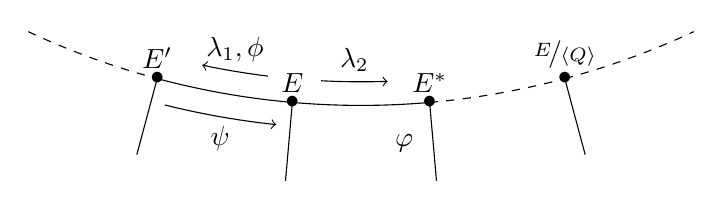
\begin{tikzpicture}[scale=1]
\coordinate (A) at (245:10);
\coordinate (B) at (255:10);
\coordinate (B') at (255:11);
\coordinate (B1) at (256:10.3);
\coordinate (C) at (265:10);
\coordinate (C') at (265:11);
\coordinate (D) at (275:10);
\coordinate (D') at (275:11);
\coordinate (E) at (285:10);
\coordinate (E') at (285:11);
\coordinate (F) at (295:10);
\coordinate (F') at (295:11);
\coordinate (G) at (305:10);
\coordinate (B2) at (258:9.7);
\coordinate (C1) at (266:10.3);
\coordinate (C2) at (267:9.7);
\coordinate (encre) at (273:10.5);
\draw (A) arc(245:255:10)[dashed];
\draw (B) arc(255:275:10);
\draw (D) arc(275:285:10)[dashed];
\draw (E) arc(285:295:10)[dashed];
\draw (B) node[above] {$E'$} node{$\bullet$};
\draw (C) node[above] {$E$} node{$\bullet$};
\draw (D) node[above] {$E^*$} node{$\bullet$};
\draw (E) node[above] {$\nicefrac{E}{\langle Q \rangle }$} node{$\bullet$};
\draw (encre) node {$\varphi$};
\draw (B)--(B');
\draw (C)--(C');
\draw (D)--(D');
\draw (E)--(E');
\draw (B1) arc(256:264:10.3) [->] node[below,midway] {$\psi$}; %flèche représentant \psi
\draw (B2) arc(258:263:9.7) [<-] node[above,midway] {$\lambda_1, \phi$}; %flèche représentant 
\draw (C2) arc(267:272:9.7) [->] node[above,midway] {$\lambda_2$}; %flèche représentant 
% \draw (C1) arc(266:284:10.3) [->];% node[below,midway,fill=white] {$\varphi $};

%\draw (260:10.75) node{}
%\draw (0,0) arc (245:255:10)[dashed] node[above] {$C$} node{$\bullet$} --(0:1.5);
%\draw (0,0) arc (245:255:10)[dashed] arc (255:265:10) node[above] {$E^i$} node{$\bullet$} --(0:1.5);
%\draw (-1,0) arc (245:255:10) node[above] {$C2$} node{$\bullet$} --(90:1)[color=yellow];
%\draw (-1,0) arc (245:255:10) node[above] {$C$} node{$\bullet$} --(310:1.5)[color=red];
%\draw (0,0) arc (245:255:10)[color=white] node[above] {$C$} node{$\bullet$} arc (255:265:10) node[above] {$E^i$} node{$\bullet$} arc (265:275:10) node[above] {$E$} node{$\bullet$} arc (275:285:10) node[above] {$F$} node{$\bullet$} arc (285:295:10) node[above] {$G$} node{$\bullet$} ; 
\end{tikzpicture}
\end{center}
\caption{ Example for the case $\ell=2$ } 
\end{figure}
\begin{algorithm}
\caption{\label{alg:horizontal}Computing a horizontal point of order~$ℓ^k$}
% Horizontalisation of $R$ following the $\lambda$ direction}
\begin{algorithmic}[1]
\REQUIRE $(P_0, Q_0)$: a diagonal basis of~$E[ℓ^{h+1}]$; $k$: an integer.\\
% $R$: a point of~$E$ of order $ℓ^k$ such that
% $ℓ^n R$~is horizontal of direction~$μ$ for some~$n ≤ k$.
\ENSURE $R$: a horizontal point of~$E[ℓ^k]$ with direction~$λ$.
\FOR{$i = 1$ to~$k-1$}
\STATE $ϕ_i \gets $ isogeny with kernel~$\chev{ℓ^{h} P_{i-1}}$
\STATE $Q_{i} \gets ϕ_i(Q_{i-1})$
\STATE $P' \gets \mathsf{divide}(\ell, ϕ_i(P_{i-1}))$.
\STATE Write~$π(P') = λ P' + b Q_i$ for~$b ∈ ℤ/ℓℤ$ and
let $P_{i} \gets P' - (b/μ) Q_i$.
\ENDFOR
\RETURN $R = \widehat{ϕ}_1 ∘ … ∘ \widehat{ϕ}_{k-1}
  (\mathsf{divide}( ℓ^{k-(h+1)}, P_{k-1}) )$. 
% \RETURN $\{\widehat{ϕ}_1,..,\widehat{ϕ}_n\}, R_n, P_n$
\end{algorithmic}
\end{algorithm}
\begin{prop}
Algorithm~\ref{alg:horizontal} is correct and has a complexity of
% The computation complexity of algorithm \ref{alg:diagonal} is
%\begin{equation*}
%\begin{array}{ll}
%O\pa{\cout{M}(ℓ^k) · k · (k + \log q)}, &\text{if $ℓ = 2$;}\\
%O\pa{\cout{M}(ℓ^k) · ℓ^k · k^2 · \log ℓ · \log q
%  \;+\; k · \cout{F}(q, ℓ^k)}, &\text{if $ℓ ≠ 2$.}
%\end{array}
%\end{equation*}
\begin{equation*}
O(k(\mathsf{R}(k-\beta)))
\end{equation*}
\end{prop}
\begin{proof}
We check that at step~$i$ of the loop,
the points~$(P_i, Q_i)$ form a diagonal basis of~$E_i[ℓ^{h+1}]$,
and $ϕ_i$~has direction~$λ$.
The fact that $R$~is horizontal is then a consequence
of Proposition~\ref{prop:push-horizontal}.
% the point $ℓ^{n-i} R_i$ is horizontal with direction~$μ$,
% using Proposition~\ref{prop:push-horizontal} for the induction step.
% Since $ϕ_{i+1}$ is horizontal with direction~$λ$,
% according to Proposition~\ref{prop:push-horizontal},
% $ℓ^{n-i-1} R_{i+1} = ϕ_{i+1} (ℓ^{n-i-1} R_i)$ is also horizontal
% with direction~$μ$.
The complexity analysis %of Algorithm~\ref{alg:horizontal}
is exactly the same as for Algorithm~\ref{alg:diagonal}.
\end{proof}

% After execution of Algorithm~\ref{alg:horizontal},
% the point~$P_n$ is horizontal
% 
% In practice, we shall use Algorithm~\ref{alg:horizontal}
% in the case where~$R = Q_{k}$ as output from Algorithm~\ref{alg:diagonal}.
% In that case, since $Q_k$~is diagonal, $ℓ^{h} Q_k$~is horizontal,
% so that we may use~$n=h$.
One application of Algorithm~\ref{alg:diagonal} (with input~$k ← h+1$)
and two applications of Algorithm~\ref{alg:horizontal} allow us
to compute a horizontal basis of~$E[ℓ^k]$.
This could be done directly with Algorithm~\ref{alg:diagonal} instead,
but that would require computing in an extension $F_{k+h-\beta}$.
%of degree up to~$ℓ^{k+h}$.

%Algorithme necessaire, surement pour enfoncer le clou...


%%%%%%%%%%%%%%%

\section{Interpolation step}
\label{sec:interpolation}

After constructing bases $(P,Q)$ of $E[ℓ^k]$ and $(P',Q')$ of
$E'[ℓ^k]$ using the algorithms of the previous section, our algorithm
computes the polynomial with coefficients in $\F_q$ sending
$x(P)↦x(P')$, $x(Q)↦x(Q')$, and the other abscissas accordingly.  In
this section we give an efficient algorithm for this specific
interpolation problem. The algorithm has already appeared
in~\cite{df10} and~\cite{enge+morain03}; we briefly recall it here,
and adapt the complexity analysis to out setting.

\subsection{Interpolating a polynomial on a field extension}

We start by tackling a simpler problem. We suppose we have constructed
a tower of Kummer extensions $\F_q=F_0⊂F_1⊂\cdots⊂F_n$, with
$[F₁:F₀]\mid(ℓ-1)$, and $[F_{i+1}:F_i]=ℓ$ for any $i>0$. Given two
elements $v,w∈F_n\setminus F_{n-1}$, we want to compute polynomials
$T$ and $L$ such that:
\begin{itemize}
\item $T \in \F_q[x]$ is the minimal polynomial of $v$, of degree
  $d=\deg T<ℓ^n$;
\item $L$ is in $\F_q[x]$, of degree less than $d$, and $L(v)=w$.
\end{itemize}
Observe that, since $v,w∉F_{n-1}$, we necessarily have $v_ℓ(d)=n-1$,
so that $ℓ^{n-1}≤d<ℓ^n$.

Using a fast interpolation algorithm~\cite[Chapter~10.2]{vzGG}, the
polynomials $T$ and $L$ could be computed in
$O\bigl(n\MM(ℓ^{2n})\log(ℓ)\bigr)$ operations in $\F_q$. We can do
much better by exploiting the form of the Kummer tower, and the
Frobenius algorithm given in Lemma~\ref{lemma:frob-ell}.

Following~\cite{df10}, we first compute $T$, starting from
$T^{(0)}=x-v$.  We let $\sigma_i$ be the map that takes all the
coefficients of a polynomial in $F_{n-i}[x]$ to the power
$\#F_{n-i-1}$. For $i=0,\dots,n-2$, suppose we know a polynomial
$T^{(i)}$ of degree $\ell^i$ in $F_{n-i}[x]$. Then, compute the
polynomials $T^{(i,j)}$ given by
\begin{equation*}
  T^{(i,j)}= \sigma_i^j\bigl (T^{(i)} \bigr)
  \quad\text{for $0 \le j \le \ell-1$},
\end{equation*}
and define
$$T^{(i+1)}=\prod_{j=0}^{\ell-1} T^{(i,j)};$$ one easily sees that
$T^{(i+1)}$ is the minimal polynomial of $v$ over $F_{n-i+1}$. For the
last step $i=n-1$, we proceed in a similar way by defining
\begin{equation*}
  T = T^{(n)}=\prod_{j=0}^{d/ℓ^{n-1}} T^{(n-1,j)}.
\end{equation*}

\begin{lem}\label{lemma:interpolation:minpoly}
  The cost of computing $T^{(n)}=T$ is bounded by
  $O\bigl(nℓ\bigl(\MM(ℓ^{n+1}) + \MM(ℓ)\log(q)\bigr)\bigr)$ operations in $\F_q$.
\end{lem}

\begin{proof}
  At each step $i$, from the knowledge of $T^{(i)}$ we compute all
  $T^{(i,j)}$ using Lemma~\ref{lemma:frob-ell}. The cost for a single
  polynomial $T^{(i,j)}$ is of
  $O\bigl(ℓ^i\bigl(ℓ^{n-i}\MM(ℓ)+\MM(ℓ^{n-i})\bigr)\bigr)$ operations,
  which we simplify to a total of $O(ℓ\MM(ℓ^{n+1}))$ for all $O(\ell)$
  of them.

  At each step, we must also account for the precomputation required
  by Lemma~\ref{lemma:frob-ell}, which costs $O(ℓ\MM(ℓ)\log(q))$
  operations.

  From the $T^{(i,j)}$'s we compute $T^{(i+1)}$ using a subproduct
  tree, as in~\cite[Lemma~10.4]{vzGG}. The result has degree
  $O(ℓ^{i+1})$ and coefficients in $F_{n-i}$, thus the overall cost is
  $O(\MM(ℓ^{n+1})\log(ℓ))$. After $T^{(i+1)}$ is computed this way, we
  can convert its coefficients to $F_{n-i-1}$ at no algebraic cost.

  Summing over all $i$, we obtain the stated complexity.
\end{proof}

We can finally proceed with the interpolation itself. First, compute
$w' = w/T'(v)$ and let $L^{(0)}=w'$.  Next, for $i=0,\dots,n-2$,
suppose we know a polynomial $L^{(i)}$ in $F_{n-i}[x]$ of degree less
than $\ell^i$. We compute the polynomials $L^{(i,j)}$ given by
$$L^{(i,j)}= \sigma_i^j\bigl(L^{(i)}\bigr),$$
for $0 \le j \le \ell-1$, and
$$L^{(i+1)} = \sum_{j=0}^{\ell-1} L^{(i,j)}\frac{T^{(i+1)}}{T^{(i,j)}}.$$ The last step $i=n-1$
is done analogously.  As shown in~\cite{df10}, $L^{(n)}$ is the
polynomial $L$ we are looking for.

\begin{prop}
  Given elements $v,w∈F_n\setminus F_{n-1}$, the cost of computing the
  minimal polynomial $T∈\F_q[x]$ of $v$, and the interpolating
  polynomial $L∈\F_q[x]$ such that $L(v)=w$, is of
  $O\bigl(nℓ\bigl(\MM(ℓ^{n+1}) + \MM(ℓ)\log(q)\bigr)\bigr)$ operations
  in $\F_q$.
\end{prop}
\begin{proof}
  After the polynomials $T^{(i)}$ have been computed, we need to
  compute $T'(v)$. This is done by means of successive Euclidean
  remainders, since
  $T'(v) = (((T' \bmod T^{(1)}) \bmod T^{(2)}) \cdots \bmod T^{(n)})$.
  At stage $i$, we have to compute the Euclidean division of a
  polynomial of degree $O(ℓ^{n-i+1})$ by one of degree $O(ℓ^{n-i})$ in
  $F_i[x]$. Using the complexities from Section~\ref{sub:towers} we
  deduce that each division can be done in time $O(\MM(ℓ^{n+1}))$, for
  a total of $O(n\MM(ℓ^{n+1}))$ operations. Then, computing
  $w' = w/T'(v)$ takes $O(\MM(\ell^n)\log(\ell^n))$ operations.

  Finally, at each step $i$, the polynomials $L^{(i,j)}$ are computed
  at a cost of $O(ℓ\MM(ℓ^{n+1}))$, as in the proof of
  Lemma~\ref{lemma:interpolation:minpoly}.  The computation of
  $T^{(i)}$ requires $O(ℓ)$ additions, multiplications and divisions
  of polynomials of degree $O(ℓ^{i+1})$ with coefficients in
  $F_{n-i}$, again at a cost of $O(ℓ\MM(ℓ^{n+1}))$. Summing over all
  $i$, the complexity statement follows readily.
\end{proof}

\section{The complete algorithm}
\label{sec:complete-algorithm}
%%%%%%%%%%%%%%%
\subsection{Finding a suitable $ℓ$-volcano}
\label{sub:shape-volcano}

Our algorithm uses an Elkies prime~$ℓ$.
According to Chebotarev's density theorem,
\todo{apparemment selon qu'on transcrit depuis le russe ou l'ukrainien
son nom change, je voudrais ne pas trop troller le referee si possible}
the density of primes~$ℓ$ such that~$(d_K/ℓ) = +1$ is asymptotically~$1/2$,
so that we need only try a $O(1)$ number of primes~$ℓ$.
Since~$d_K$ is not assumed to be known yet,
we need to be able to compute the shape of the crater,
as well the shortest $ℓ$-isogeny chain from~$E$ to the crater.

\todo{Eventually explicit the complexity of computing a shape of the volcano i.e. $\mathcal{F}(\ell)$}
% One crucial point before starting to use methods described above is to determine if the input curves of problem \ref{prob:isogeny-problem} are located on a cylic crater of a volcano and if it is not the case compute a the shortest chain of $\ell$-isogeny to a curve on the crater. 
%   \newline
As we will need to compute the $\ell^{\infty}$ rational torsion of the curve, we start by doing it using algorithm like \ref{alg:diagonal}, and then we take advantage of this knowledge like in \cite{MireMRV05} \todo{check this quote} to build an ascending path until we reach a level of stability where there is no more link between the structure of the $\ell^{\infty}$ rational torsion of a curve and its level in the volcano. After this we use methods like in \cite{volcano} to find a curve on the crater by exploring all the chain of $\ell$-isogenies. In the case where the volcano has no level of stabilty (said regular) then we have a cost of $O(\frac{\log(q)}{\log(\ell}) \mathsf{R}(1) )$ otherwise it is of  $O( ( \frac{\log(q)}{\log(\ell})^2 \mathcal{F}(\ell) )$, with $h=O(( \frac{\log(q)}{\log(\ell}))$ the height of the volcano (not known a priori) and $\mathcal{F}(\ell)$ the cost of computing roots of a $\ell$ modular polynomial of $O(\ell^2+M(\ell)\log(q))$. 
\newline
Once we got a curve on the crater we still have to determine which kind of crater the curve is located on. Using algorithm \ref{alg:diagonal} we can compute a matrix of the Frobenius on the $\ell^{h+1}$ torsion , since we know $h$ the height of the volcano, if we got two distinct eigenvalues then the crater is cyclic otherwise it is not. The classical method from \cite{volcano} is to look for  the length of $(\ell+1)$ descending chain of $\ell$-isogenies on the volcano, if there is two paths of length greater than the others then the crater is cyclic, if not the crater is not cyclic. This is done in a complexity of $O( ( \frac{\log(q)}{\log(\ell})\ell \mathcal{F}(\ell) )$. We can also mention methods used in \cite{IonicaJ10} which are done in a complexity of $O(h(\ell^3+\ell \mathsf{M}(\ell) \log(q)))=O(( \frac{\log(q)}{\log(\ell})(\ell^3+\ell \mathsf{M}(\ell) \log(q)))$ and take advantage of the structure of the $\ell$ torsion when it is linked with the level in volcano with pairings that determine ascending or horizontal $\ell$-isogenies. %when the curve is not located over a stability level.
\newline 
For $\ell=2$ we can use methods like in \cite{MiretMRV05}. The height and the shape of the volcano can be computed with a complexity of $O(\log^6(q))$ which computes an ascending path and can determine the shape of the crater by taking advantage of the torsion structure when it is linked with the level in volcano otherwise it uses methods similar to \cite{volcano}.
 %c est exactement ce qui est fait dans ce papier...
  
\subsection{Lifting the problem to a cyclic crater}

If the two input curves~$E$, $E'$ of our algorithm
belong to cyclic $ℓ$-isogenies volcanos but not to their crater,
then by Proposition~\ref{prop:parallel},
their depth below the craters is the same.
Using the methods of~\ref{sub:shape-volcano},
we can compute the shortest path of $ℓ$-isogenies~$α: E → E_{\max}$,
$α': E' → E'_{\max}$ linking the curves~$E, E'$ to the craters.
By Proposition~\ref{prop:parallel} (iii),
the curves~$E_{\max}$ and~$E'_{\max}$ are again $r$-isogenous;
we can use our algorithm to compute such an isogeny~$ψ_{\max}$.
Then $ψ = (α')^{-1} ∘ ψ_{\max} ∘ α$ is the required $r$-isogeny.

 \subsection{Curves which are on the cyclic crater}
 % The previous sections \ref{sec:acti-frob-endm}, \ref{sec:interpolation} describe steps of the algorithm for curves located on the crater of cyclic volcano (Elkies) and 
 The previous subsection describe how to reduce the problem to the case of elliptic curves located on a cyclic crater of a volcano. Thus for this subsection we consider two input curves $E$, $E'$ at the problem \ref{prob:isogeny-problem} in this situation. We will work with $\ell^{k}$ torsion point with $k$ such that $k \geqslant h+1$ and such that $(\ell^2-1)\ell^{2k-2}> 8 r$, the first condition is necessary to compute horizontal $\ell$-isogenies, the second one is necessary to have enough points for the interpolation of the $r$-isogeny. We can notice that the first condition is only necessary for section \ref{sec:acti-frob-endm}, we can then work only with horizontal points of degree $\ell^k$ such that they verify $(\ell^2-1)\ell^{2k-2}> 8 r$.

In this section we work with the abscissas of points of order $\ell^k$ on two input
curves $E,E'$ as in Problem~\ref{prob:isogeny-problem}, with $k$ fixed.
As input, we are given horizontal bases $(P,Q)$ of $E[\ell^k]$ and
$(P',Q')$ of $E'[\ell^k]$ as computed in
Section~\ref{sec:acti-frob-endm}, together with two coefficients $(a,b)
\in \left(\mathbb{Z}/\ell^k \mathbb{Z} \right)^{\times}$. For the discussion below,
let $S$ and $S'$ denote the set of abscissae of points of order
$\ell^k$ on respectively $E$ and $E'$.

The algorithm in this section computes two polynomials. The first of
them is $T(x)$, which is the squarefree monic polynomial whose roots
are the elements in $S$; in particular, it does not depend on
$E'$. More crucially, we also compute an interpolation polynomial
$L(x)$ that maps $S$ to a permutation of $S'$ induced by the mapping
$P \mapsto aP'$ and $Q \mapsto bQ'$.  Precisely, this means that we
ask that $L(x(cP+dQ))=x(caP'+dbQ')$ holds for all pairs $(c,d) \in
(\mathbb{Z}/\ell^k\mathbb{Z})^2$ for which either $c$ or $d$ is
coprime with $\ell$, in which case $cP+dQ$ and $acP'+dbQ'$ have order
$\ell^k$; here, $x(P)$ denotes the abscissa of a point $P$.

As before, \todo{really? where?} we assume that $\pi(P)=\lambda P$ and
$\pi(Q) = \mu Q$, with $\lambda \bmod \ell = \mu \bmod \ell = 1$ and $\lambda \neq \mu \bmod \ell^k$.  We
further let $\alpha$ and $\beta$ be the respective multiplicative orders %$\ell$-adic valuations 
of $\lambda$ and $\mu$ as defined in \ref{prop:degree-l-torsion}.%\todo{Wrong it is their $\ell$-adic 
%valuation of their multiplicative order modulo $\ell^k$ } 

\begin{defi}
For $u,v$ in $\{0,\dots,k-1,k\}$, we denote by $T_{u,v}$ the set
of all points on $E$ of the form $R=c P + d Q$, with $(c,d)$ in
$(\Z/\ell^k\Z)^2$, $c$ and $d$ having respective $\ell$-adic
valuations $u$ and $v$ (having valuation $k$ means that the
corresponding element is zero). All these points are in $E[\ell^k]$
\end{defi}

The set of points of order exactly $\ell^k$ is the disjoint union of
the sets $T_{u,v}$ for which either $u$ or $v$ is zero.

Take $u,v$ as above. For $R$ in $T_{u,v}$ and $s \ge 0$, we have
$\pi^s(R) = c\lambda^s P+ d \mu^s Q$.  Because $\lambda$ and $\mu$ are
both equal to $1$ modulo $\ell$, the set $T_{u,v}$ is thus the
disjoint union of orbits under the action of $\pi$. For any $R$ as
above, the length of its orbit (which is as well the degree of its
field of definition over $\F_q$ \todo{replace with $F_1$}) is the least $s>0$ such that $c
\lambda^s = c \bmod \ell^k$ and $d \mu^s =d \bmod \ell^k$. It is thus
given by $\ell^e$, with $e={\max(k-u-\alpha, k-v-\beta, 0)}$. %if I am
%not wrong.

\begin{prop} \label{prop:cout-repre}
The cost of computing all the representatives of points of order $\ell^k$ is of $O(\M(\ell^{2k})\log(\ell^k))$.
\end{prop}

\begin{proof}
To get representatives of these orbits, we start by computing
$\ell^uP$ and $\ell^vQ$. They have respective degrees
$\ell^{\max(k-u-\alpha, 0)}$ and $\ell^{\max(k-v-\beta, 0)}$ over
$\F_q$, and to simplify matters we assume that they are both given
over $\F_{q^{\ell^e}}$. This can be done in $O( \M(\ell^k)
\log(\ell^k))$ operations in $\F_q$. \todo{explain, projective
  coordinates}. Next, we compute representatives $C_{u,v} \subset
U=(\Z/\ell^{k-u}\Z)^{\times} \times (\Z/\ell^{k-v}\Z)^{\times}$ for the cosets
modulo $(\lambda, \mu)$; $C_{u,v}$ has cardinality $(\ell-1)^2
\ell^{2k-u-v-2-e}$. This is done in a direct manner, by a loop over
all elements in $U$ (for any element not marked before, we add it to
the representatives and mark all elements in its coset); this takes
$O(\ell^{2k-u-v})$ multiplications  in $U$, each of which can be
done in quasi-linear bit complexity in $\log(\ell^k)$.

Finally, we compute the sequence $R_{u,v}=(R_{u,v,c,d}\ \mid (c,d) \in
C_{u,v})$, with $R_{u,v,c,d}=c \ell^u P + d \ell^v Q$; these points
are all defined over $\F_{q^{\ell^e}}$ and there are $(\ell-1)^2
\ell^{2k-u-v-2-e}$ of them. This takes $O(\ell^{2k-u-v-e}
\M(\ell^e)\log(\ell^k))$ operations in $\F_q$, which is $O(\ell^{-u-v}
\M(\ell^{2k})\log(\ell^k))$. Summing over all $u,v$ 
(with either $u=0$ or $v=0$) leads to a total
of $O(\M(\ell^{2k})\log(\ell^k))$.

\end{proof}

We do the same thing on $E'$ using $aP'$ and $bQ'$ instead of $P$ and
$Q$, computing points $R'_{u,v}$. Then, we apply the algorithm of 
the previous section to each pair $(R_{u,v,c,d},R'_{u,v,c,d})$. \todo{discuss
the fact that we take only abscissae; maybe $\ell=2$ needs special case}
This takes $O(\M(\ell^e)\log(\ell^e))$ operations in $\F_q$ per point,
for a total of $O( \ell^{-u-v} \M(\ell^{2k})\log(\ell^k))$ as above.
Summing over all $u,v$ 
(with either $u=0$ or $v=0$) leads to a total
of $O(\M(\ell^{2k})\log(\ell^k))$.
\todo{work out all this stuff precisely, and don't forget the bit complexity of 
finding representatives}

After we are done with all $u,v$'s, we are left with polynomials
$(T_{u,v,c,d},L_{u,v,c,d})$ with coefficients in $\F_q$ that describe
the restriction of the mapping we want to recover to the corresponding
orbits. We apply the Chinese Remainder Theorem to compute a unique
pair $(T,L)$ that describes the action of the putative isogeny over
all points of order $\ell^k$. The CRT takes time
$O(\M(\ell^{2k})\log(\ell^k))$, since the sum of the lengths of the
orbits is less than $\ell^{2k}$.

\begin{prop} \label{prop: cout-interp}
The cost of computing the polynomials $(T,L)$ is of $O(k\ell\mathsf{M}(\ell^{2k+1})+\mathsf{\ell}\log(q))$ with precomputations of $O(\M(\ell^{2k})\log(\ell^k))$ in $\mathbb{F}_q$
\end{prop}

 
%%  We work with the points of order $\ell^k$ on two input
%% curves $E,E'$  with $k$ fixed.%as in Problem~\ref{prob:isogeny-problem}, that lie on
%% %the cyclic crater of a volcano of $\ell$-isogenies (in all this
%% %section, $k$ is fixed).
%% As input, we are given horizontal bases $(P,Q)$ of $E[\ell^k]$ and
%% $(P',Q')$ of $E'[\ell^k]$ as computed in
%% Section~\ref{sec:acti-frob-endm}, together with two coefficients $(a,b)
%% \in \left(\mathbb{Z}/\ell^k \mathbb{Z} \right)^{\times}$. For the discussion below,
%% let $S$ and $S'$ denote the set of abscissae of points of order
%% $\ell^k$ on respectively $E$ and $E'$.

%% The algorithm in this subsection computes two polynomials. The first of
%% them is $T(x)$, which is the squarefree monic polynomial whose roots
%% are the elements in $S$; in particular, it does not depend on
%% $E'$. More crucially, we also compute an interpolation polynomial
%% $L(x)$ that maps $S$ to a permutation of $S'$ induced by the mapping
%% $P \mapsto aP'$ and $Q \mapsto bQ'$.

%% Precisely, this means that we ask that $L(x(cP+dQ))=x(caP'+dbQ')$
%% holds for all pairs $(c,d) \in (\mathbb{Z}/\ell^k\mathbb{Z})^2$ for
%% which either $c$ or $d$ is coprime with $\ell$, in which case $cP+dQ$
%% and $acP'+dbQ'$ have order $\ell^k$; here, $x(P)$ denotes the abscissa
%% of a point $P$.  
%% \newline
%% \begin{prop}
%% The points of order $\ell^k$ of $E$ are of order $\ell^{k-\beta} \leqslant \ell^i \leqslant \ell^{k-\alpha} $ for the Frobenius action according to the structure of $E[\ell^\infty](\F_k)$.
%% \newline
%% The sets of points of orders $\ell^k$ and of order $\ell^i$ for the Frobenius are of size less than $\ell^{2k}\frac{\ell^{i}}{\ell^{k-\beta}}$ and have at most $\ell^{k+\beta}$ representatives.
%% \end{prop}
%% The computations of representants of the different orbits is done working only with indexes in $(\mathbb{Z}/\ell^k \mathbb{Z}^{\times})^2$ of the basis $(P,Q)$. Once we have the indexes we compute the corresponding points. We state the following result on the cost of computing all of them:

%% \begin{prop}%\todo{a verifier plus en detail..., voir si on peut pas se servir de la proposition de Jerome}
%% The cost of computings the different representatives of orbits is majorated by  $O(\ell^{k}M(\ell^{k})k \log(\ell))$.
%% \end{prop}

%% \begin{proof}
%% %We have at most $\ell^{2k}\frac{\ell^{i}}{\ell^{k-\beta}\ell^i}$ points of order $\ell^k$ representatives 
%% %of orbits of order $\ell^i$ for the Frobenius with 
%% For each of the representatives we have up to $k \log(\ell)$ operations to compute them. Overall we have a complexity $k\log(\ell) \ell^{k+\beta} \sum_{i=\beta}^{\alpha}\mathsf{M}(\ell^{k-i})$. Let $c$ be such that we can multiply elements of $\mathbb{F}_{q^{\ell^{k-i}}}$ in $c\ell^{k-i}(k-i)\log(k-i)$ majorated by $c\ell^{k-i}(k)\log(k)$, then we get $\sum_{i=\beta}^{\alpha}c\ell^{k-i}(k)\log(k) \leqslant c\ell^{k-\beta+1}(k)\log(k)$. In the end we get the cost majorated by $c\ell^{k+\beta}\ell^{k-\beta+1}(k)\log(k)k\log(\ell)=c\ell^{k}\mathsf{M}(\ell^{k})k\log(\ell)$
%% \end{proof}
%% We then have to apply the results of the preceding section to compute for each representative of orbits of order $\ell^i$ their interpolation polynomial associated.

%% \begin{prop}
%% With the knowledge of the representatives of different orbits we can compute the interpolations polynomials with a complexity of $O(\mathsf{M}(\ell^{2k})k\log(k))$
%% \end{prop}

%% \begin{proof}
%% Since we have at most $\frac{\ell^{2k}}{\ell^{k-\beta}}$ representatives of orbits of points of order $ \ell^{k-\beta} \leqslant \ell^i \leqslant\ell^{k-\alpha}$ for the Frobenius. From \todo{mettre reference au dernier resultat de section 4} we have an overall complexity of $\ell^{k+\beta}\sum_{i=k-\alpha}^{k-\beta}M(\ell^i)\log(\ell^i)$. Let $c$ be such that the cost of computing an interpolation polynomial is less than $c\ell^ik\log^2(k)\log(\log(k))$, we then have the total cost less than $c\ell^{k+\beta}\ell^{k-\beta+1}\log^2(k)\log(\log(k))k$. 
%% \end{proof}

%% We recombine then all those interpolations polynomials using Chinese Remainder Theorem. %We can notice also that the modulus for the Chinese Remainder Theorem do not depend of the choices of the coefficients $(a,b) \in (\mathbb{Z}/\ell^k \mathbb{Z}^*)^2$ for the interpolation, thus we can use this to speed up the next occurrences of the CRT by doing precomputation for the inverse of the modulus in the CRT, we state thus two complexity analysis for the CRT .

%% \begin{prop}
%% The cost of the C.R.T. applied on all the different orbits for the first occurence is of $O(M(\ell^{2k})\log(\ell^{2k}))$ operations in $\mathbb{F}_q$. %For the next occurences the cost is of $O(M(\ell^{2k})\log(\ell^{k+\alpha}))$ operations in $\mathbb{F}_q$.
%% \end{prop}

%% \begin{proof}
%% The assertion comes from the fact that there is $\ell^{2k-2}\frac{\ell^2-1}{\ell^2}$ points of order $\ell^k$ and we work with polynomials in $\mathbb{F}_q[x]$. %The second one comes from the fact that we have $\ell^{k+\alpha}$ representatives of orbits and we do only multiplication and additions on the polynomials associated to the orbits, we conclude by lemma \ref{lemma:mul-pol}
%% \end{proof}

%% \begin{prop}
%% The total cost of computing polynomials $L$, $T$ is of $O(\mathsf{M}(\ell^{2k})k\log(k))$ with $O(\ell^k\mathsf{M}(\ell^k)k\log(l))$ precomputations independent from the choices of the interpolation mapping coefficients $a,b$. 
%% \end{prop}

%\todo{Do it by splitting the set of $\ell^k$ torsion into orbits for
 % the Frobenius. Each orbit can be handled in quasi-linear time using
 % the previous subsection, and the recombination is just Chinese
 % remaindering over $\F_q$, so we should be good.}

%\todo{Make sure that computing one representative per orbit is not too
 % expensive.}

\todo{complete the complexity}
 To complete the complexity analysis we need to state the complexity of solving a division polynomial of degree $\ell^2$ in the aim of computing a basis of the $\ell$ torsion to apply algorithms of $\ell$ division. It has a complexity of $O(M(l)\log(\ell) \ell^5 \log(\ell^2) \log(q))$, using Cantor-Zassenhauss in $F_1$. %with $d$ the order of $q$ in $\mathbb{Z}/\ell\mathbb{Z}^*$.%Cantor Zassenhauss dans F_1
 %Then we use algorithm \ref{alg:diagonal} to obtain a diagonal basis $(P,Q)$ of the $\ell^k$ torsion with a complexity of $O(k(\mathsf{R}(k)+\mathsf{F}(k,0)))$. 
 \newline
  Now we are able to describe the entire algorithm,   
  as like the Couveignes' algorithm we proceed in 3 steps to solve problem \ref{prob:isogeny-problem}:
 \begin{enumerate}
\item Compute horizontal basis $P,Q$ and $P',Q'$ of
  $E[\ell^k]$ and $E'[\ell^k]$ respectively, for $\frac{3}{2}\ell^{2k-2} > 4r$ \todo{preciser cette borne ??} ;
\item\label{alg:modif-couveignes:interp} Choose $(a,b) \in (\mathbb{Z}/\ell^k\mathbb{Z}^*)^2$ and compute the interpolation
  polynomial $L$ \todo{(verify that notation is consistent
    with Sec.4)} sending $x(P)$ to $x(aP')$ and $x(Q)$ to $x(bQ')$, and the abscissas of
  their scalar multiples of order $\ell^k$ accordingly;
\item\label{alg:modif-couveignes:rational} Deduce a rational fraction
  congruent to $L$ modulo $T$, and verify that it
  defines an isogeny of degree $r$. If it does, return it, otherwise
  replace $P',Q'$ with an other horizontal basis of $E'[\ell^k]$ and go back to
  Step~\ref{alg:orig-couveignes:interp}.
\end{enumerate} 

\begin{prop}
The complexity of solving problem \ref{prob:isogeny-problem} for two elliptic curves located on a cyclic crater of volcano of $\ell$-isogeny is of $O(rM(r)\log(r))$ in $\mathbb{F}_q$ plus a pre-computation of $O(\mathsf{M}(r)\log(r))$
\end{prop}

\begin{proof}%refaire ça avec les notations de Luca
We just have to multiply by $r$ the results obtained from \ref{prop: cout-interp} for the different try for the mapping.
\end{proof}
  
\section{Experimental results}
\label{sec:implem}

\todo{Describe implementation and show benchmarks. Possibly compare
  with Lercier-Sirvent (Luca has an implementation somewhere).}

\begin{acknowledgements}
  We thank many people.
\end{acknowledgements}

\bibliographystyle{alpha}
\bibliography{refs}


\appendix
\section{Isogenies and the Tate module}
\label{ap:Tate}
We recall here a few results about $ℓ^n$-isogenies
and the $ℓ$-adic Tate module.

The isogeny determined by a point~$P$ of order~$ℓ^n$ only depends on
the subgroup~$\chev{P}$ generated by~$P$ in~$E[ℓ^n]$.
Equivalently, this subgroup defines a point in
the projective space of~$E[ℓ^n]$,
which is a projective line over~$ℤ/ℓ^n ℤ$.

There exists a canonical bijection~\cite[II.1.1]{SL2} between
this projective line and
the set of lattices of index~$ℓ^n$ in the $ℤ_ℓ$-module $T_ℓ(E)$:
it maps a line~$\chev{P}$ to the lattice~$Λ_P = \chev{P} + ℓ^n T_ℓ(E)$.
This lattice is also the preimage by the isogeny~$ϕ_P: E → E_P$
of the lattice~$ℓ^n T_ℓ(E_P)$.

\medbreak
If a basis~$(R, S)$ of~$E[ℓ^n]$ is fixed and~$P = a R + b S$,
then the lattice~$Λ_P$ is generated by the columns of the matrix
$L_P = \smat{ℓ^n & 0 & a\\0 & ℓ^n & b}$.
Write~$b = ℓ^m b'$ with~$ℓ ∤b'$; the Hermite normal form of~$L_P$
is $M_P = \smat{ℓ^{n-m} & a/b' \\ 0 & ℓ^m}$,
and its columns also generate the lattice~$Λ_P$.
We check that $M_P$ has determinant~$ℓ^n$.
Since $Λ_P = ϕ_P^{-1} (ℓ^n T_{ℓ} (E_P))$,
there exist bases of~$T_ℓ(E), T_ℓ(E')$
in which $Φ_P$ has the matrix~$ℓ^n M_P^{-1}$.
Therefore, in that basis of~$T_ℓ(E_P)$,
the matrix of~$π|T_ℓ(E_P)$ is $M_P^{-1} · π · M_P^{}$.

\section{Division of a point by~$\ell$}
\label{ap:division}

We write~$Q ← \sfdiv{ℓ, P}$ for the computation of a preimage of~$P$
by multiplication by~$ℓ$.
The obvious way to compute~$\sfdiv{ℓ, P}$ would be to use
the $ℓ$-division polynomial.
However, this polynomial has a degree~$O(ℓ^2)$.
Instead, we factor the multiplication-by-$ℓ$ map
as a product of an $ℓ$-isogeny and its dual.
This brings the polynomial degree down to~$O(ℓ)$.
According to subsection~\ref{sub:towers},
the cost of the $\sfdiv{ℓ, P}$ operation is therefore $\mathsf{R} (k)$.
%\begin{equation}\label{eq:div-by-l}
%O \pa{\cout{M}(ℓ^k) \,· \,\left\lbrace\begin{array}{ll}
%(k + \log q) & \text{if $ℓ = 2$,} \\
%(ℓ^k · k · \log ℓ · \log q) & \text{if $ℓ ≠ 2$.}
%\end{array}\right\rbrace}.
%\end{equation}
% \begin{equation}\label{eq:div-by-l}
% \mathsf{R}(k)
% \end{equation}

\begin{algorithm}
\caption{\label{ldivision}Compute the preimage of $Q$ by the multiplication by $\ell$.}
\begin{algorithmic}[1]
\REQUIRE  $(P_1,P_2)$ a basis of $E[\ell]$;\\
$Q$: a point on $E$ such that there exist a $\ell$ division point of $Q$.
\ENSURE $Q_1$: a point on $E$ such that $\ell Q_1 = Q$.
%\STATE compute $ (P_1,P_2)$ a basis of $ E[\ell]$
\STATE $\phi_1$ $\leftarrow$ the isogeny with kernel~$\chev{P_1}$.
\STATE $\phi_2$ $\leftarrow$ the isogeny with kernel~$\chev{\phi_1(P_2)}$.
\STATE $Q_2 \leftarrow$ preimage of $Q$ by $\phi_2$
\STATE $Q_1 \leftarrow$ preimage of $Q_2$ by $\phi_1$
\RETURN $Q_1$
\end{algorithmic}
\end{algorithm}


\goodbreak
\section{Galois orbits in~$E[ℓ^k]$: the $ℓ=2$ case}
\label{ap:orbites-2-torsion}

\begin{prop}\label{prop:orbites-2-torsion}
Let~$E$ be an elliptic curve with $2$-maximal endomorphism ring.
Assume $λ ≡ μ ≡ 1 \pmod{4}$ and let~$α = v_2(λ-1), β=v_2(μ-1)$.
Write~$ν_2(x, y) = \min (x+y, x+β-2, y+α-2)$
and~$ρ_2(x, y) = x+y - ν_2(x, y) = \max (0, x-α+2, y-β+2)$.
The decomposition of the group~$E[2^k]$ in Galois orbits is as follows:
\begin{enumerate}
\item for~$i, j = 0, …, k-2$:
$4 · 2^{ν_2(i,j)}$ orbits of size~$2^{ρ_2(i,j)}$;
\item for~$i = 0, …, k-2$:
$8 · 2^{\min (i, α-2)}$ orbits of size~$2^{\max (0, i-α+2)}$;
\item the four singleton orbits of $2$-torsion points.
\end{enumerate}
\end{prop}
Note that if $λ$ or~$μ ≡ -1 \pmod{4}$ then
by replacing the base field by a quadratic extension,
we can always ensure that the condition $λ ≡ μ ≡ 1 \pmod{4}$ is
satisfied.
\begin{proof}
The proof is much the same as that of Prop.~\ref{prop:orbites-l-torsion}.
The case~$ℓ = 2$ of~\cite[Théorème II.3.2]{Serre.Arith}
states that $f(x,y,z) = 2^x · (-1)^y · \exp (4z)$
is an isomorphism between~$ℤ × (ℤ/2ℤ) × ℤ_2$ and~$ℚ_2^×$.
Let~$V(i, c)$ be the image modulo~$2^k$ of~$f(k-2-i, c, -)$;
then $V(i, c) ≃ ℤ/2^{i} ℤ$ for~$i ≥ 0$,
while~$V(-1, 0) = V(-1, 1)$ is the singleton $\acco{2^{k-1}}$.

Let~$P, Q$ be diagonal generators of~$E[2^{k}]$
and define~$W(i,j,c,d) = V(i,c) P + V(j,d) Q$;
also write~$λ = f(0,0,2^{α-2} u)$, $μ = f(0,0,2^{β-2} v)$.
Then the Galois orbits in~$W(i,j,c,d)$ correspond to $ℤ_2^2$ modulo
the lattice~$Λ_{i,j} = \smat{2^{i}&0&2^{α-2} u\\0&2^{j}&2^{β-2} v}$.
We find that $Λ_{i,j}$ has covolume~$2^{ν_2(i,j)}$.
This gives the orbits of point~(i) of the proposition.

By considering the orbits of~$V(i,c) P + ε Q$ and~$ε P + V(i,c) Q$
for~$ε ∈ \acco{0, 2^{k-1}}$, we obtain the orbits
of point~(ii).
\end{proof}
\end{document}
%  LocalWords:  isogeny morphisms Isogenies isogenies isogenous
%  LocalWords:  cardinality bijection Couveignes automorphism

% vim: ts=2:
%  LocalWords:  Frobenius endomorphism precomputation
